\section{Síntesis de voz hablada}


\subsection{Compresión y Síntesis de Señal de Voz}

Se pide aplicar compresión y síntesis la señal de voz $test\_signal$. Los pasos para realizar lo anterior corresponden a:
\begin{itemize}
    \item Compresión:
    \begin{enumerate}
        \item Subdividir la señal en segmentos de 20 ms.
        \item Obtener el valor RMS de cada segmento.
        \item Clasificar cada segmento como V, U o S con el criterio basado en RMS obtenido en la parte 2.
        \item Obtener los valores del filtro AR que simula el tracto vocal por medio de $mylpc$ para los sonidos de tipo V y U.
    \end{enumerate}
    \item Síntesis:
    
    Se van generando los segmentos en orden
    \begin{itemize}
        \item En el caso de que un segmento corresponda a un sonido S, generar segmento de silencio (ceros) de 20 ms.
        \item En el caso de que el sonido corresponda a un sonido V, excitar filtro AR respectivo con tren de impulsos de 20 ms (en este caso de 100 Hz).  Realizar corrección de RMS del segmento.
        \item En el caso de que el sonido corresponda a un sonido U, excitar filtro AR respectivo con señal de ruido blanco de 20 ms.  Realizar corrección de RMS del segmento.
    \end{itemize}
    Finalmente se concatenan los segmentos generados
\end{itemize}

El código que realiza lo anterior corresponde a \texttt{p3\_1.m} y se adjunta a la entrega.
 
El gráfico de la señal original y la sintetizada se muestran en la figura \ref{fig:p3_1}. Visualmente la síntesis parece correcta.

\begin{figure}[H]
    \centering
    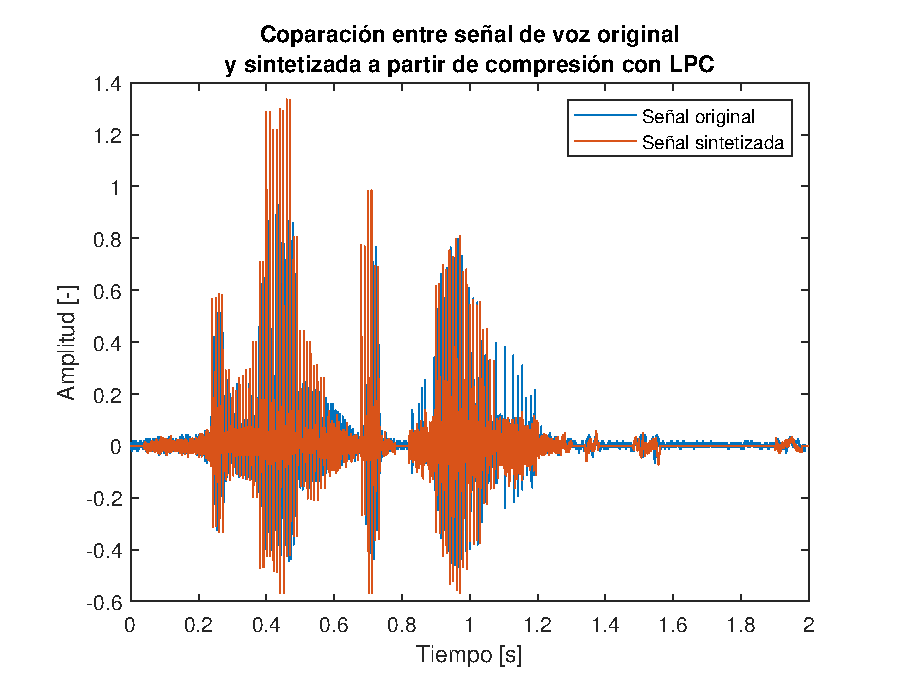
\includegraphics[width = .9\linewidth]{figures/p3_1.eps}
    \caption{Comparación gráfica de señal de voz original y sintetizada.}
    \label{fig:p3_1}
\end{figure}

Finalmente se guarda la señal sintetizada como $my\_test\_signal.wav$, la cual se adjunta a la entrega. Con respecto a la calidad del audio, si bien mantiene el timbre ''robótico'', se entiende lo que se esta diciendo. 

Para mejorar la síntesis se podría reconocer la frecuencia fundamental de la voz en sonidos tipo V y U, con la idea de excitar el filtro AR con un tren de impulsos de frecuencia acorde al hablante, obteniendo una voz más natural.

\subsection{Estimación de Compresión}

Se estima la compresión del archivo de audio como la razón entre los bytes usados para almacenar los coeficientes del filtro, los flags VUS y el valor RMS con respecto a los bytes de la señal $test\_signal$. Para lo anterior se utilizó el comando $whos$

Por lo tanto, la razón de compresión $R$ corresponde a:
$$ R = \dfrac{\text{bytes}(A) + \text{bytes}(flags) + \text{bytes}(RMSs)} {\text{bytes}(test\_signal)} = \dfrac{9088 + 100 + 100}{127360} \approx  0.079$$